% figures/ownership-map.tex
% Ownership lanes: Swage, upstream MLIR and LLVM, and PyTorch, with
% one launch traced across the three domains.
\documentclass[tikz,border=10pt]{standalone}
% figures/common-preamble.tex
% Shared setup for the TikZ documentation figures. Colors mirror the
% palette in scripts/render_docs_diagrams.py so both atlases match.
\usepackage[T1]{fontenc}
\usepackage{lmodern}
\usepackage{tikz}
\usepackage{pgfplots}
\pgfplotsset{compat=1.18}
\usetikzlibrary{arrows.meta}
\usetikzlibrary{backgrounds}
\usetikzlibrary{calc}
\usetikzlibrary{decorations.pathreplacing}
\usetikzlibrary{fit}
\usetikzlibrary{positioning}

\definecolor{swcanvas}{HTML}{FFFDF8}
\definecolor{swpanel}{HTML}{F5F3ED}
\definecolor{swink}{HTML}{17212B}
\definecolor{swmuted}{HTML}{4B5563}
\definecolor{swline}{HTML}{59636E}
\definecolor{swblue}{HTML}{00689D}
\definecolor{swbluefill}{HTML}{DCEFFD}
\definecolor{swpurple}{HTML}{8E4775}
\definecolor{swpurplefill}{HTML}{F7E2EF}
\definecolor{sworange}{HTML}{A94500}
\definecolor{sworangefill}{HTML}{FCE5DC}
\definecolor{swgreen}{HTML}{00664B}
\definecolor{swgreenfill}{HTML}{DDF4EB}
\definecolor{swgrayfill}{HTML}{EEF0F2}

\pagecolor{swcanvas}
\AtBeginDocument{\color{swink}}

\tikzset{
  swcell/.style={
    draw, minimum width=0.46cm, minimum height=0.46cm, inner sep=0pt,
    line width=0.7pt, rounded corners=1pt},
  swbox/.style={
    draw=swline, fill=swpanel, rounded corners=6pt, line width=0.9pt},
  swarrow/.style={-{Stealth[length=6pt]}, draw=swline, line width=1pt},
  swtag/.style={
    draw, rounded corners=8pt, line width=0.9pt,
    font=\bfseries\scriptsize, inner xsep=8pt, inner ysep=4pt},
  swtitle/.style={anchor=west, font=\Large\bfseries, text=swink},
  swsubtitle/.style={anchor=west, font=\small, text=swmuted},
  swcode/.style={font=\small\ttfamily, text=swink},
  every picture/.style={line cap=round},
}

\begin{document}
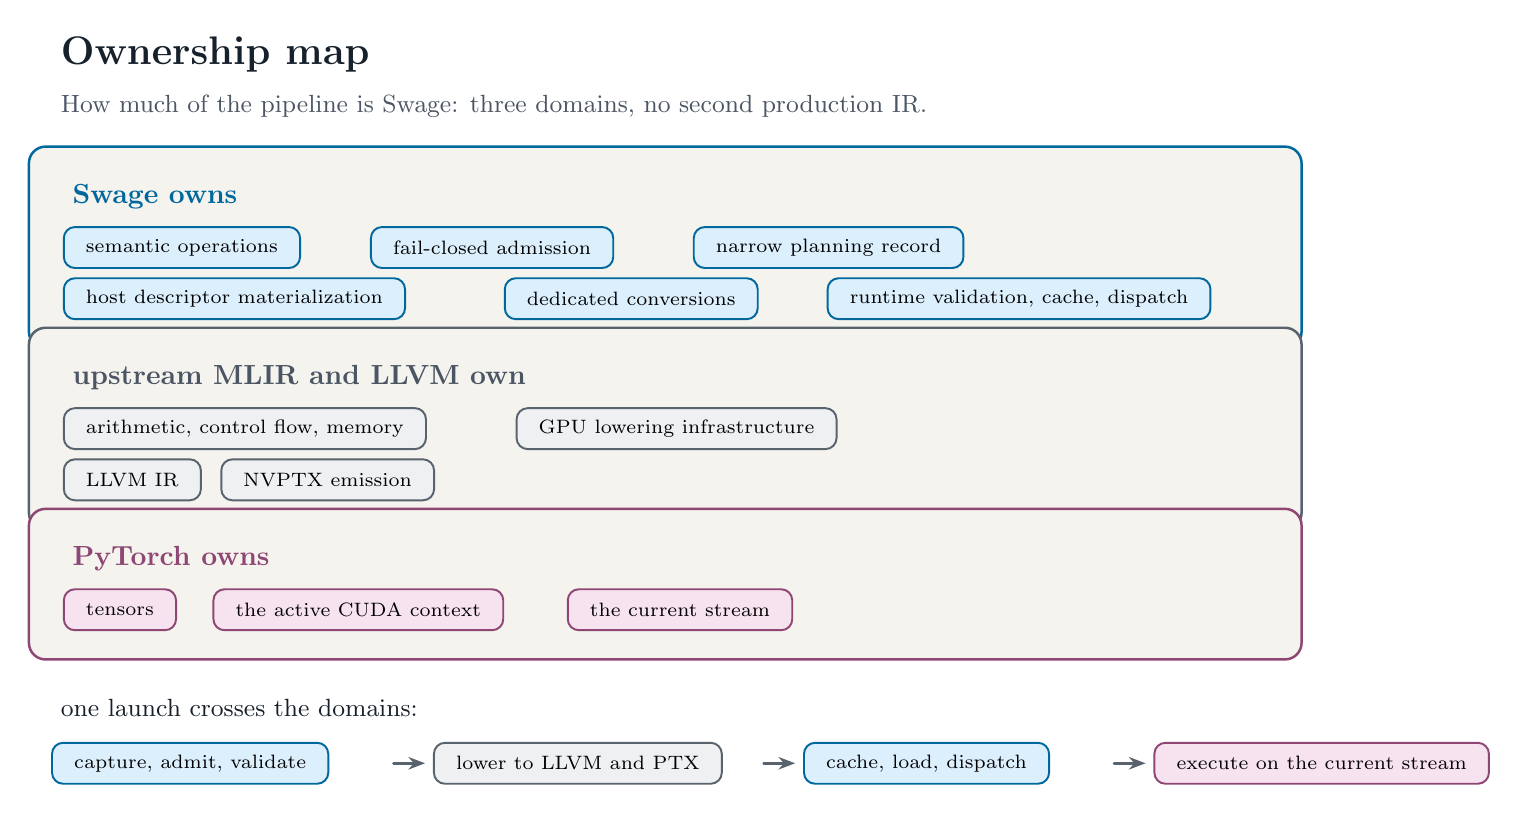
\begin{tikzpicture}[x=1cm, y=1cm,
  ownchip/.style={swcell, minimum height=0.52cm, inner xsep=8pt,
    rounded corners=4pt, font=\scriptsize}]

% Header.
\node[swtitle] at (0, 1.15) {Ownership map};
\node[swsubtitle] at (0, 0.5)
  {How much of the pipeline is Swage: three domains, no second
   production IR.};

% Swage lane.
\node[swbox, draw=swblue, fit={(0, -2.3) (15.6, -0.3)},
      inner sep=8pt] {};
\node[anchor=west, font=\bfseries, text=swblue] at (0.15, -0.65)
  {Swage owns};
\node[ownchip, fill=swbluefill, draw=swblue, anchor=west]
  at (0.15, -1.3) {semantic operations};
\node[ownchip, fill=swbluefill, draw=swblue, anchor=west]
  at (4.05, -1.3) {fail-closed admission};
\node[ownchip, fill=swbluefill, draw=swblue, anchor=west]
  at (8.15, -1.3) {narrow planning record};
\node[ownchip, fill=swbluefill, draw=swblue, anchor=west]
  at (0.15, -1.95) {host descriptor materialization};
\node[ownchip, fill=swbluefill, draw=swblue, anchor=west]
  at (5.75, -1.95) {dedicated conversions};
\node[ownchip, fill=swbluefill, draw=swblue, anchor=west]
  at (9.85, -1.95) {runtime validation, cache, dispatch};

% Upstream lane.
\node[swbox, fit={(0, -4.6) (15.6, -2.6)}, inner sep=8pt] {};
\node[anchor=west, font=\bfseries, text=swmuted] at (0.15, -2.95)
  {upstream MLIR and LLVM own};
\node[ownchip, fill=swgrayfill, draw=swline, anchor=west]
  at (0.15, -3.6) {arithmetic, control flow, memory};
\node[ownchip, fill=swgrayfill, draw=swline, anchor=west]
  at (5.9, -3.6) {GPU lowering infrastructure};
\node[ownchip, fill=swgrayfill, draw=swline, anchor=west]
  at (0.15, -4.25) {LLVM IR};
\node[ownchip, fill=swgrayfill, draw=swline, anchor=west]
  at (2.15, -4.25) {NVPTX emission};

% PyTorch lane.
\node[swbox, draw=swpurple, fit={(0, -6.25) (15.6, -4.9)},
      inner sep=8pt] {};
\node[anchor=west, font=\bfseries, text=swpurple] at (0.15, -5.25)
  {PyTorch owns};
\node[ownchip, fill=swpurplefill, draw=swpurple, anchor=west]
  at (0.15, -5.9) {tensors};
\node[ownchip, fill=swpurplefill, draw=swpurple, anchor=west]
  at (2.05, -5.9) {the active CUDA context};
\node[ownchip, fill=swpurplefill, draw=swpurple, anchor=west]
  at (6.55, -5.9) {the current stream};

% One launch crosses the three domains in order.
\node[anchor=west, font=\small, text=swink] at (0, -7.15)
  {one launch crosses the domains:};
\node[ownchip, fill=swbluefill, draw=swblue, anchor=west]
  at (0, -7.85) {capture, admit, validate};
\draw[swarrow] (4.35, -7.85) -- (4.75, -7.85);
\node[ownchip, fill=swgrayfill, draw=swline, anchor=west]
  at (4.85, -7.85) {lower to LLVM and PTX};
\draw[swarrow] (9.05, -7.85) -- (9.45, -7.85);
\node[ownchip, fill=swbluefill, draw=swblue, anchor=west]
  at (9.55, -7.85) {cache, load, dispatch};
\draw[swarrow] (13.5, -7.85) -- (13.9, -7.85);
\node[ownchip, fill=swpurplefill, draw=swpurple, anchor=west]
  at (14.0, -7.85) {execute on the current stream};

\end{tikzpicture}
\end{document}
